\chapter{Evaluation}
\label{chapter:evaluation}

Kata Containers hardens the security of containerized environment by adding the extra layer of security with the micro VM. The architectural change and new components of the environment enable the additional security features. These components, such as the micro VM and hypervisor, come with a price of degraded performance and computational overhead. Previous work, such as \cite{EverartsdeVelp2020} and \cite{Kumar2020} have examined the performance when compared Kata Containers against the native runtime runC, the most common OCI-compliant runtime. In these two papers, Kata Containers architecture design results in a performance decrease in IO throughput and overhead in memory and CPU utilization. However, the results in these papers are highly dependant on the underlying test environment. These tests do not consider the latest development and performance optimization of Kata Containers' performance. This paper evaluates the system performance in an environment simulating a telco edge cloud architecture and regular workload.

\section{Test architecture}
\label{section:test_architecture}

Telco applications are relying on high-performing and optimized computing. The ever-more increasing performance requirements from users add a great demand on the underlying infrastructure. Software and hardware-based architectural changes to the edge cloud environment need to be carefully evaluated before implementing them into the production. It might otherwise stall the performance and significantly decrease the performance for mobile network users.

The test environment, visualized in Figure \ref{fig:TestArchitectureCluster}, is a simple single-node cluster with one container. The main focus of the tests is to evaluate the impact of Kata Containers and the choice of the hypervisor to I/O operations throughput and latency on various storage methods, such as PV, emptyDir, and hostPath. The full test combination matrix is described in Table \ref{table:TestMatrix}. The tests also measure CPU and memory overhead of Kata Containers architecture in general. The test cluster is hosted on K3s\cite{K3s} version 1.17.3, which is a lightweight version of Kubernetes supporting the identical API. K3s is Kubernetes distribution built for IoT and edge computing with a lower footprint on memory and disk usage. K3s uses containerd as a native container runtime engine. Due to compatibility issues, Kata Containers uses version XXX.

\begin{figure}[ht]
  \begin{center}
    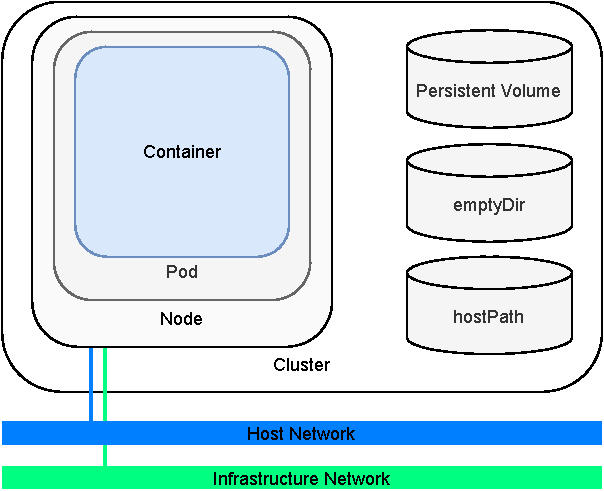
\includegraphics[width=12cm]{images/TestArchitectureClusterSimple.pdf}
    \caption{Kubernetes test cluster overview}
    \label{fig:TestArchitectureCluster}
  \end{center}
\end{figure}

\section{Methodology}

The tests of this thesis aim to measure the possible performance degradation of I/O operations and additional CPU and memory resource consumption due to the Kata Containers architecture. A dedicated server
hosts the test environment, and it is built and tailored to support edge and far edge cloud deployments. The server includes an Intel Xeon 6212U CPU with 24 cores and 48 threads with x86 architecture at 2.40 GHz clock-speed and 192GB of DDR4 memory at 2933 MHz clock speed, which is shared to the cluster.

The performance tests run with Fio \cite{FIO}, an I/O performance tester intending to simulate a variety of I/O workloads without resorting to writing tailored test cases repeatedly. Fio supports various test configurations such as multiple threads, block sizes, I/O sizes, and I/O patterns. In this thesis, the tests are time-based, where each test runs for 30 seconds. The file size of each writable file is 2 GB. The Fio job file is described in Appendix \ref{appendix:fio_jobfile}. Each test is repeated three times, and averaging the results. Table \ref{table:TestMatrix} describes the test combination matrix. In the tests, each possible combination is sampled, resulting in 1632 different test scenarios. 

\begin{table}[ht]
\centering
\caption{Test combinations matrix}
\vspace{\baselineskip}
\begin{tabular}{| c | c | c | c | c |}
\hline
\textbf{Runtime} & \textbf{Jobs} & \textbf{Block size} & \textbf{I/O pattern} & \textbf{I/O device} \\ 
\hline
Bare metal & 1 & 512 & read & emptyDir (memory) \\
\hline
runC & 2 & 1024 & write & emptyDir (disk) \\ 
\hline
CLH & 3 & 2048 & randread & local (PV) \\
\hline
QEMU & & 4096 & randwrite & hostPath \\
\hline
QEMU VirtioFS & & 8192 & & \\
\hline
& & 16384 & & \\
\hline
& & 32768 & & \\
\hline
& & 65536 & & \\
\hline
\end{tabular}
\label{table:TestMatrix}
\end{table}

The test matrix consists of five columns: runtime, jobs, block size, I/O pattern, and I/O device, the runtime of the tests refers to the container runtime or hypervisor. In the case of bare metal, the test is run on the host without containerization. In bare-metal test runs, the performance test is launched with CPU affinity to an isolated CPU with taskset \cite{taskset} command. Jobs refer to the number of concurrent clones. Each clone of the job is spawned as an independent thread or process. Block size is the size in bytes for I/O units applying for reads and writes. I/O pattern has sequential and random pattern reads and writes. I/O type of the test is buffered. I/O device refers to the storage media used for the test destination. EmptyDir is created on the container, whereas the host maintains local Persistent Volume and hostPath.

Fio test suite is wrapped inside a Docker image with a Linux OS Alpine \cite{Alpine}, which aims to deliver general-purpose Linux with security, simplicity, and resource efficiency. The tests are deployed with Helm\cite{Helm}, a package manager for Kubernetes helping with the deployment of applications. The Kubernetes Pods are deployed as Guaranteed Quality-of-Service with two CPUs and 18GB of memory to support the tests. However, each Kata Containers VM and runC container gets assigned with only 1 CPU. This restriction allows comparing tests to bare metal tests, which are run on an isolated single CPU environment. The system performance, to measure CPU and memory overhead, is logged with Prometheus and Grafana.

\section{Results}

Each test is run on isolated resources, and final results are averaged out of three tests. Fio provides a comprehensive catalog of parameters as test results, of which the most important ones are completion latency, IOPS, and IO throughput. Completion latency describes the completion time in milliseconds for key percentiles such as 50\% and 99.99\%. IOPS is the number of I/O operations per second. IO throughput or bandwidth in megabytes per second is the sum of block size multiplied by IOPS. Bare-metal test results work as a benchmark of the best-case scenario.

Previous work \cite{EverartsdeVelp2020}\cite{Kumar2020}\cite{StackHPCKata}\cite{Randazzo2019} on measuring Kata Containers' performance resulted in highly unified performance between bare-metal and runC. In read and write tests, runC slightly outperformed the tested Kata Containers setups with faster throughput and lower resource usage. However, the results of these papers varied due to the diversity in underlying infrastructure and the difference in test frameworks. None of these researches tested the whole spectrum of hypervisors and various storage options offered in the Kubernetes environment.

\subsection{I/O performance}

The hypervisor of Kata Containers adds its overhead to the performance. The main focus of I/O tests is to evaluate the performance of Kata Containers with various hypervisors against the runC runtime and determine the inherent performance metrics of each hypervisor. As described in Table \ref{table:TestMatrix}, the test includes three different Kata Containers hypervisors: CLH, QEMU, and QEMU with virtio-fs.

\subsection{Storage performance}

Kubernetes offers multiple storage options for various deployments, and each of these options offers slightly different performance and features. The tests include four storage options suitable for the telco environment: disk and memory-based emptyDir, hostPath as Persistent Volume, and hostPath. The main focus is to evaluate these storage methods concerning block sizes between 512 bytes and 64 KBs and concurrent jobs from one to three. It is essential to make the distinction of evaluating the best option for non-persistent and persistent volumes.

\subsection{CPU performance}

The architectural design of Kata Containers adds extra components to the system. Each of these components adds overhead to the CPU performance via background processes. In the CPU performance tests, the main question was to measure the overhead and the need for extra cores compared to runC. The measurement of CPU performance was implemented by creating workloads and recording the performance with Prometheus. 

2 cores allocated (1 for workload, 1 for general)

\subsection{Memory performance}

Memory overhead

\section{Evaluation}

\textcolor{red}{Results?}
\textcolor{red}{What the results mean?}